\documentclass[11pt,twocolumn]{article} 

\usepackage[spanish]{babel}
\usepackage{url, hyperref}
\usepackage{tabularx}
\usepackage{graphicx}
\DeclareGraphicsExtensions{.png}
\title{
\vspace{-3cm}   
Sistemas de Autentificaci\'on
}

\author{ 
Jorge Rubens Lipa Challapa\\
Edgar Jose Valencia Cayetano\\
Ronald Heredia Camacho\\
Fernando Solis Tapia\\
\\
Universidad Mayor de San Sim\'on \\
Sociedad Cient\'ifica de Estudiantes de Sistemas e Inform\'atica\\
\url {http://www.scesi.org/}
}

\date{ \today }

\begin{document}
\maketitle

\begin{abstract} 
Los sistemas de autentificaci\'on ofrecen un control de 
acceso para un grupo determinado de personas y ofrecer datos estad\'isticos 
referentes a las entradas y salidas del personal donde se procesara para 
proveer informaci\'on muy valiosa al momento de realizar seguimiento, 
frecuencia de accesos y controlando los permisos de acceso al ambiente.\\
\\
 Pudiendo ser utilizado en diferentes en diferentes \'ambitos y \'areas de
 trabajo donde se requiera autentificaci\'on digital.
\end{abstract}

\section{Introducci\'on}
Uno de los problemas de seguridad mas frecuentes,  a sido el control de acceso 
a ambientes que requieren de una identificaci\'on. Esto se puede deber a  la 
cantidad de usuarios que se maneja, tama\~no del ambiente o el tipo de acceso. 
Las diferentes soluciones existentes llegan a tener alg\'un tipo de dificultad, 
ya sea por tiempo, costo y tambien sobre el personal encargado donde la 
implementaci\'on llega a ser laboriosa y compleja para los encargados.\\
\\
Los sistema de autentificacion basados en RFID, 
permitir\'an, el manejo y control de personal y seguimiento de actividades a
 todo usuario que necesite una verificaci\'on de identidad para ingresar a un
 ambiente o consumir un servicio utilizando tecnolog\'ias como \textit{Android,
 Arduino y Servicios web} esto permitir\'a que un encargado de seguridad o 
gesti\'on pueda pueda administrar el control de acceso del personal de una 
manera r\'apida y simple a un costo reducido.\\

\section{Antecedentes}

Generalmente se ve muy a menudo que todos los ambientes  con un nivel de acceso 
tengan una seguridad de acuerdo a un est\'andar , para dar cierta privacidad y 
confidencialidad, esto puede variar ya que los dispositivos de acceso pueden o 
no hacer un seguimiento de las actividades sobre el personal. Esto deja al 
descubierto agujeros de seguridad en el ambiente, que mas tarde se interpretara 
como debilidades y falencias en la seguridad.\\
\\
Para asegurar la confidencialidad y privacidad, de ambientes que requieran un 
control de acceso limitando a un grupo de personas, se llega a la conclusi\'on: 
Estos individuos  requieren de permisos especiales, en este caso roles de 
acceso, para ingresar o realizar actividades que est\'en limitadas por un 
dispositivo de control. \\

\section{RFID}

RFID, Radio Frequency Identification permite transmitir la identidad de un 
objeto a una frecuencia con que se comunica con un dispositivo que reconoce al 
objeto. Este comportamiento esta basado en el modelo emisor receptor. \\

\begin{figure}[t]
  \begin{center}
    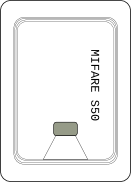
\includegraphics[width=2in]{mifare.png}
  \end{center}

  \caption{\small Dise\~no interno de Mifare S50.}
  \label{fig-label}
\end{figure}

\section{Mifare S50}

La tarjeta plástica PVC laminada tamaño ISO estándar: 85,7 x 54 x 0,82 mm, 6gr. aprox, trabaja a una frecuencia: 13,56 MHz integrado a un Chip Mifare de lectura y escritura la velocidad de transferencia para la lectura y escritura esta establecida a unos 106 Kbits/s. Esta tarjetas como sus predecesoras viene  con 1Kbytes de memoria EEPROM, de los cuales estan disponibles en 16 sectores y asignados con un n\'umero de serie \'unico de 4 bytes. Este n\'umero ya viene incluido desde fabrica.\\
\\
La distancia m\'axima para realizar una lectura o escritura es de 10 cm, los datos pueden permanecer almacenados por al menos 10 a\~nos. \\
\\
Tal como se muestra en la Figura 1. El esquema de la tarjeta esta dividido en dos partes:\\

\begin{itemize}
	\item Antena de cobre
	\item Chip Mifare.
\end{itemize}

La funcionalidad de esta tarjeta varia en funcionalidad, como ser: para autentificaci\'on, y monetizaci\'on. En la actualidad varios pa\'ises emplean de diferentes formas el uso de los dispositivos de identificicaci\'on, como venta de pasajes para autobuses, identificacion en tarjetas de credito, credenciales medicas. inventarios de productos y ganado.\\ 

\section{Aporte tecnol\'ogico}

La implementaci\'on de hardware libres como Arduino impulsara la adopci\'on de los dispositivos electr\'onicos en otras \'areas gracias a la gran variedad de m\'odulos que cuenta y tambi\'en tecnolog\'ias como los servicios web que descentralizaran la informaci\'on y el monitoreo en tiempo real, permitiendo a diferentes dispositivos tener informaci\'on de manera inmediata mediante celulares, tablets, paginas web.\\
\\
Para ello los proyectos Centinela y PocketPay, proponen una posible soluci\'on al control de acceso y monetizaci\'on utilizando RFID como base.\\

\section{Proyecto Centinela}

Centinela, Control y seguimiento de actividades de acceso para la identificaci\'on de personal. Basado en tecnolog\'ias  open source. Dicho sistema  proveer\'a el acceso a ambientes controlados mediante RFID, los datos ser\'an mandados mediante un servicio web para su procesamiento en un servidor.  Figura \ref{fig-centinela}.\\
\\
Los datos obtenidos se utilizaran para realizar reportes de seguimiento a los usuarios registrados. Los dispositivos de recolecci\'on estan basados en dise\~no construidos con arduino, mientras  que para los dispositivos m\'oviles que tengan NFC se manejaran mediante una aplicaci\'on movil que se conectara con el servicio web.\\

\begin{figure}[!h]
  \begin{center}
    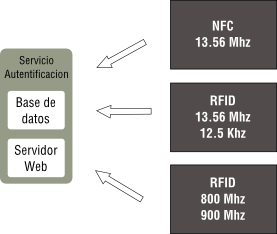
\includegraphics[width=2in]{architect.png}
  \end{center}

  \caption{\small Modelo de implementaci\'on para el Proyecto Centinela.}
  \label{fig-centinela}
\end{figure}

\section{Proyecto PocketPay}

Orientado a la cargar y recargar de cr\'edito, utilizando la funcionalidad 
"Wallet" (monedero) de las tarjetas Mifare S50. Con esto se podr\'a realizar 
el intercambio de cr\'edito que se asociara a un monto de dinero, pudiendo 
representar una forma de pago o cambio, por ejemplo en un auto bus, pagar 
los pasajes con una identificaci\'on RFID, recargar cr\'editos en un vale 
de descuento y dem\'as usos que tenga que ver con cambios de estado para un 
incremento y decremento.\\

Un dispositivo de control realizara la transacci\'on y guardara los cambios en 
el dispositivo de manera r\'apida. la recargar se har\'a mediante  otro 
dispositivo que guardara los datos de usuarios y la cantidad del incremento 
o decremento.\\

Los Servicios de control se los realizara v\'ia web mediante un servicio web 
compatible con Centinela para verificar la autenticidad de la tarjeta y 
realizar el seguimiento. Figura \ref{fig-pocketpay}.\\

\begin{figure}[!h]
  \begin{center}
    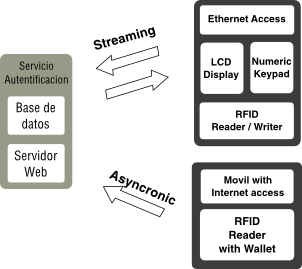
\includegraphics[width=2in]{pocketpay.png}
  \end{center}

  \caption{\small Modelo de implementaci\'on para el Proyecto PocketPay.}
  \label{fig-pocketpay}
\end{figure}


\section{Metodolog\'ia de trabajo}  

La para la realizaci\' de los proyectos citados y dar la funcionalidad 
esperada,es necesario  administrar y gestionar la informaci\'on de los usuarios y los 
dispositivos de control.

La metodolog\'ia de trabajo se apoyara en la siguientes historias para un posterior 
desarrollo, estas  comprende tres \'areas  que dar\'an como resultado a un 
sistema de autentificaci\'on:\\

	\subsection{ Sistema web }
	
	\begin{description}
		\item [Registro basado en roles] Gesti\'on de los usuarios como el 
		administrador, seguridad y personal com\'un.
		\item [Dispositivos de control] Gesti\'on de los dispositivos de control.
		\item [Seguimiento] Seguimiento de las actividades referentes a las 
		credenciales de autentificaci\'on.
		\item [Reportes de seguimiento] An\'alisis de datos referentes a las 
		actividades de los usuarios autentificados.
	\end{description}
	
	\subsection{Aplicaci\'on m\'ovil}		
	
	 \begin{description}
		 \item[Seguimiento de actividad] Seguimiento de procesos de identificaci\'on 
		 a los dispositivos de control.
		 \item[Reporte personal] Reporte de seguimiento de actividad personal.
	 \end{description}
	
	\subsection{Dispositivo electr\'onico}
	
	 \begin{description}
		 \item[Comunicaci\'on con sistema web] Interfaz de acceso al sistema web 
		 mediante una conexi\'on Ethernet.
		 \item[Verificaci\'on de identidad] Control de acceso mediante RFID.
		 \item[Interacci\'on con usuario] Estado de verificaci\'on mediante 
		 componentes electr\'onicos.
	 \end{description}			

\section{Herramientas y dispositivos de Desarrollo}

Se a clasificado las herramientas y dispositivos que servir\'an para la 
culminaci\'on del prototipo inicial, establecidos en las secciones: Dispositivos 
electr\'onicos, Herramientas de prueba, Herramientas de desarrollo.

	\subsection{Dispositivos electr\'onicos }

	Los  dispositivos electr\'onicos que se mencionan est\'an limitados en base 
	al prototipo que se pretende realizar:\\
	
	\begin{enumerate}
		\item Arduino Uno
		\item Raspberry Pi Modelo B
		\item Tarjeta RFID Mifare S50
		\item Lector RFID RS232 13.56 Mhz
		\item M\'odulo de red (arduino) ENC28J60
		\item M\'odulo SD Card (arduino)
		\item M\'odulo Keypad (arduino)
		\item Ruteador inalambrico y red
		\item Cableado de red 
		\item Tableta o m\'ovil para el acceso al sistema
	\end{enumerate}
	
	\subsection{Herramientas de desarrollo}
	
	Esta secci\'on detalla el software que se utilizara para el desarrollo en 
	todos los ambientes de trabajo del proyecto Centinela y PocketPay ,detallando su 
	descripci\'on con la versi\'on y su desempe\~no en un ambiente de producci\'on :
	
	\begin{enumerate}
		\item Apache v2.2
		\item PHP v5.4
		\item PostgreSQL v9.3
		\item Laravel Framework v4.2
		\item Android v4.0.4
		\item Apache Cordova v3.5
		\item Arduino IDE v1.0.5
	\end{enumerate}

\section{Conclusiones y recomendaciones}

Con la ayuda de Arduino, las tecnolog\'ias de RFID llega a competir  frente a 
productos comerciales, si se compara la funcionalidad. Seg\'un la experiencia 
obtenida a lo largo del desarrollo, los  aspectos t\'ecnicos no son un impedimento 
para que surjan proyectos altamente eficientes y lucrativos  utilizando Arduino 
y su familia de m\'odulos disponibles. \\
\\	
Tanto al utilidad funcional de Centinela como PocketPay aun se encuentran en maduraci\'on donde se podr\'an ver otros aspectos relevantes donde saldr\'an nuevos proyectos de acuerdo a la adopoci\'on de RFID para su uso como sistema de autentificaci\'on, conservando as\'i el objetivo principal el de fomentar el uso de RFID y Software Libre (Open Source).\\
\\
Con estos proyectos se espera tambi\'en que la adopci\'on de RFID se propague a otros usos fuera de los sistemas de autentificaci\'on para la innovaci\'on de productos que faciliten el trabajo diario.


\section{Referencia Bibliogr\'afica}
	
	\begin{itemize}
		\item  Tedjasaputra, Adi (18 de diciembre 2006). «RFID Tag Attachments». RFID 
		Asia. Consultado el 3 de agosto 2007.
		
		\item Dargan, Gaurav; Johnson,Brian; Panchalingam, Mukunthan; Stratis, 
		Chris (2004), The Use of Radio Frequency Identification as a Replacement for 
		Traditional Barcoding
		
		\item "REST APIs must be hypertext driven by Roy Fielding". Roy.gbiv.com. 
		2008-10-20. Retrieved 2013-02-07.
		
		\item Matthieu Schapranow (2013), "Real-time Security Extensions for EPCglobal
		 Networks: Case Study for the Pharmaceutical Industry"
		 
		 \item Nemai Chandra Karmakar (2010)"Handbook of Smart Antennas for RFID 
		 Systems"
		 
	\end{itemize}
	
\end{document}          